%%%%%%%%%%%%%%%%%%%%%%%%%%%%%%%%%%%%%%%%%%%%%%%%%%%%%%%%%%%%
%%%%%%%%%%%%%%%%%%%%%%%%%%%%%%%%%%%%%%%%%%%%%%%%%%%%%%%%%%%%
\section{Building a Finite Element Space}\label{Sec:General}
%%%%%%%%%%%%%%%%%%%%%%%%%%%%%%%%%%%%%%%%%%%%%%%%%%%%%%%%%%%%
%%%%%%%%%%%%%%%%%%%%%%%%%%%%%%%%%%%%%%%%%%%%%%%%%%%%%%%%%%%%

\subsection{General Construction}

\begin{frame}
\frametitle{Introduction}
\begin{itemize}
\item We consider affine finite element spaces: 
\begin{itemize}
\item Global functions are pieced together from local functions on each element.
\item Local functions are constructed by transformation from a reference element.
\end{itemize}
\item Global functions need not be continuous and can be vector-valued.
\item The functions on the reference element are collected in the module \lstinline{dune-localfunctions}.
\item Constructing the global function spaces from this is part of PDELab.
\end{itemize}
\end{frame}


\begin{frame}
\frametitle{Finite-dimensional Function Spaces}
$\Omega\subset\mathbb{R}^n$, $n\geq 1$, is a domain, 
$\mathbb{T}_h$ a grid partitioning the domain $\Omega$.

\begin{Def}[Finite-dimensional function space]\label{Def:Vh}
\begin{equation*}\label{Eq:GenericFESpace}
\begin{split}
U_h(\mathbb{T}_h) &= \Biggl\{ u_h(x) : \bigcup_{e\in E_h^0}\Omega_e
 \to \mathbb{K}^m\,\Bigg| \\
&\quad u_h(x) = \sum_{e\in E_h^0}\sum_{i=0}^{k(e)-1} (\mathbf{u})_{g(e,i)}
\, \pi_e(\hat{x}) \, \hat\phi_{e,i}(\hat{x}) \, \chi_e(x); \, \hat{x}=\mu_e^{-1}(x) 
 \Biggr\}
\end{split}
\end{equation*}
defines a general finite-dimensional function space of element-wise
continuous functions.\hfill$\square$ 
\end{Def}
\end{frame}

\begin{frame}
\frametitle{Building Blocks}
\begin{itemize}
\item $\mathbb{K}=\mathbb{R}$ or $\mathbb{K}=\mathbb{C}$.
  $m\geq 1$ denotes vector-valued function spaces. 
\item $\hat\Omega_e$ is the \textit{reference element} associated with
element $e\in E_h^0$. $\mu_e : \overline{\hat\Omega}_e \to
  \overline{\Omega}_e$ maps the reference element to $\Omega$.
\item $\hat\Phi_e
  = \left\{\hat\phi_{e,i}: \overline{\hat\Omega}_e \to \mathbb{R}^{m'}\,|\,0\leq
  i < k(e)\right\}$ is 
  the set of \textit{local basis functions} for element $e$.
\item $\pi_e(\hat{x})\in\mathbb{R}^{m\times m'}$ is a
  transformation. A non-trivial example is the Piola
  transformation \cite{BrezziFortin}
\begin{equation*}
\pi_e(\hat{x}) = \frac{1}{\text{det}\  \nabla\mu_e(\hat{x})} \nabla \mu_e(\hat{x})
\end{equation*}
where $\nabla \mu_e$ denotes the Jacobian of the map $\mu_e$. For most
finite element spaces $\pi_e$ is just the identity and we have $m'=m$.
\item $g : L \to \mathbb{N}$, $L=\left\{ (e,i)\in E_h^0 \times
  \mathbb{N} \,|\, 0\leq i < k(e)\right\}$ is the \textit{local to global map}
  and $\mathcal{I}_{U_h} = \text{im}\,g$ is the associated \textit{global index set}.
\item $\mathbf{u}\in \mathbf{U}=\mathbb{K}^{\mathcal{I}_{U_h}}$ is a coefficient vector.
\end{itemize}
\end{frame}

\begin{frame}
\frametitle{Global Basis Functions}
For $j\in \mathcal{I}_{U_h}$ we define the \textit{global basis function}
\begin{equation*}
U_h \ni \phi_j(x) = \sum_{(e,i)\in L(j)} \pi_e(\mu_e^{-1}(x)) \,
\hat\phi_{e,i}(\mu_e^{-1}(x)) \, \chi_e(x)
\end{equation*} 
and $L(j) = \left\{ (e,i)\in L \,|\, g(e,i)=j \right\}$.
With that we have
\begin{align}
\Phi_{U_h} &= \{\phi_i \,|\, i\in \mathcal{I}_{U_h}\}, & U_h &= \text{span}\ \Phi_{U_h}.
\end{align}
and the finite element isomorphism
\begin{align}\label{Eq:FiniteElementIsomorphism}
\text{FE}_{\Phi_{U_h}} &: \mathbf{U} \to
U_h, & \text{FE}_{\Phi_{U_h}}(\mathbf{u})
&= \sum_{i\in\mathcal{I}_{U_h}} (\mathbf{u})_i \phi_i \ . 
\end{align} 

Definition \ref{Def:Vh} allows for functions that are
\textit{discontinuous} at element boundaries. 

If limits on the skeleton $\Gamma_h = \Omega\setminus \bigcup_ {e\in
  E_h^0} \Omega_e$ coincide, a function may be extended to 
$\left(C^0(\Omega)\right)^m$.
\end{frame}


\subsection{Local Finite Element Space}

A global finite element space is built up from a collection of local
finite element spaces for each element.

\begin{frame}
\frametitle{Local Finite Element Space}
A finite element space on the reference element (compare \cite{Ciarlet}) 
implements \lstinline{Dune::FiniteElementInterface}:
\begin{enumerate}
\item The type of reference element, given by \lstinline{Dune::GeometryType}.
\item The local basis functions
$\hat\Phi = \{\hat\phi_i : \mathbb{D}^n \to \mathbb{K}^m \,|\, 0\leq i < k\}$
and possibly derivatives in a class implementing e.g \lstinline{C0BasisInterface}.
\item Information that allows to construct the local to global map $g:
(e,i) \mapsto j$ in a class implementing \lstinline{Dune::LocalCoefficientsInterface}. 
\item A method that allows to compute coefficients $z_i$ such that
\begin{equation*}
\sum_{0\leq i < k} z_i \hat\phi_i = \hat{u} \qquad \hat{u}\in\text{span}\hat\Phi 
\end{equation*} 
in a class implementing
from \lstinline{Dune::InterpolationInterface}. For
$\hat{u}\not\in\text{span}\hat\Phi$ the method provides a projection.
\end{enumerate}
The dune module \lstinline{dune-localfunctions} provides a
collection of local finite element spaces.
\end{frame}

\begin{frame}[fragile]
\frametitle{Function Traits}
The local basis is required to contain a class \lstinline{Traits} that
gives the types for
$\mathbb{D}, \mathbb{D}^n, \mathbb{K}, \mathbb{K}^m$, the numbers $n$,
$m$ and a type for the Jacobian:
\begin{lstlisting}[basicstyle=\scriptsize,numbers=left, 
numberstyle=\tiny, numbersep=5pt]
template<class DF, int n, class D, class RF, int m, class R, 
         class J, int dorder=0>
struct LocalBasisTraits 
{
  typedef DF DomainFieldType;  typedef D DomainType;
  typedef RF RangeFieldType;   typedef R RangeType;

  enum { dimDomain = n }; enum { dimRange = m }; 

  typedef J JacobianType;

  enum { diffOrder=dorder };
};
\end{lstlisting}
Later on, other classes representing functions will use the same
traits classes.
\end{frame}

\begin{frame}
\frametitle{$Q_1$ Local Basis}
We now consider the bilinear elements $Q_1$ as an example.

The basis functions are given by
\begin{align*}
\hat\phi_2(\hat{x}) &= (1-\hat{x}_0)\hat{x}_1, &
\hat\phi_3(\hat{x}) &= \hat{x}_0\hat{x}_1, \\
\hat\phi_0(\hat{x}) &= (1-\hat{x}_0)(1-\hat{x}_1), &
\hat\phi_1(\hat{x}) &= \hat{x}_0(1-\hat{x}_1).
\end{align*}

\begin{columns}
\begin{column}{0.65\textwidth}
The numbering of the basis functions corresponds to the reference
quadrilateral.
\end{column}
\mode<presentation>{
\begin{column}{0.3\textwidth}
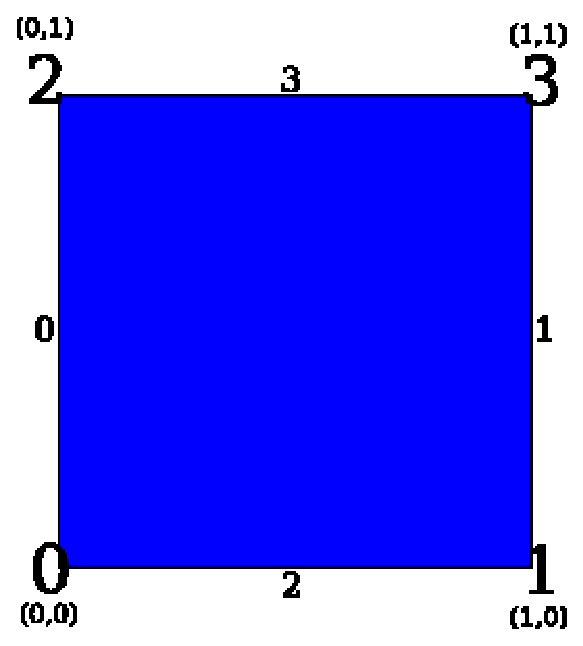
\includegraphics[width=\textwidth]{./EPS/quadrilateral}
\end{column}}
\end{columns}

\mode<article>{
\begin{figure}
\begin{center}
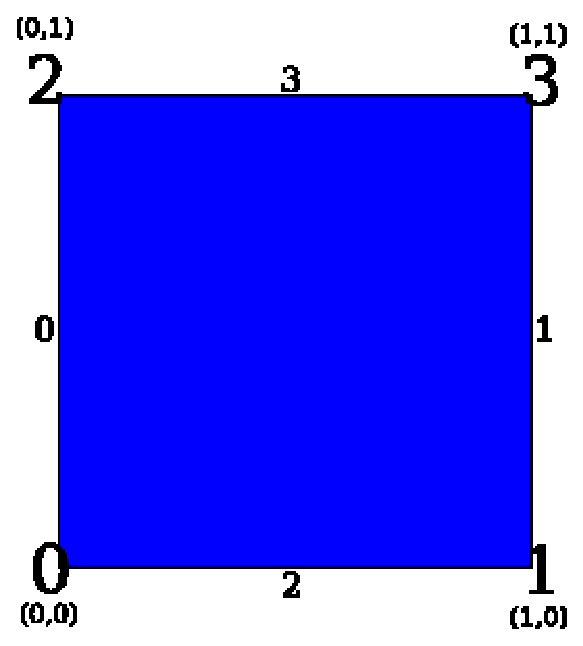
\includegraphics[width=0.5\textwidth]{./EPS/quadrilateral}
\end{center}
\caption{DUNE reference quadrilateral.}
\end{figure}}
\end{frame}

\begin{frame}[fragile]
\frametitle{$Q_1$ Local Basis Implementation}
\begin{itemize}
\item The following listing gives an implementation of the $Q_1$ local basis
functions in 2D. 
\item We provide also gradients ($C^1$ function).
\item There is also an interface for higher derivatives (not shown).
\item Evaluation always provides the values of \textit{all} basis functions
or gradients at \textit{one} point (in coordinates of the reference element). 
\item Implementations typically use \lstinline{Dune::FieldVector<T,n>} to
represent short vectors.
\item \lstinline{JacobianType} is \lstinline{Dune::FieldMatrix<R,1,2>}.
\item In the jacobian evaluation in lines \ref{q1b:grad0} to \ref{q1b:grad3}
we have
\begin{equation*}
\text{\lstinline{out[i][j][k]}}
= \partial_{\hat{x}_k} \left(\hat\phi_i\right)_j (\hat{x}) . 
\end{equation*}
\end{itemize}
\end{frame}


\begin{frame}<presentation>[fragile,allowframebreaks,allowdisplaybreaks]
\frametitle<presentation>{$Q_1$ Local Basis Listing}
\framesubtitle<presentation>{File \texttt{examples/q1localbasis.hh}}
\lstinputlisting[basicstyle=\scriptsize,numbers=left, 
numberstyle=\tiny, numbersep=5pt]{../../examples/q1localbasis.hh}
\end{frame}
\mode<article>{
\begin{Lst}[File examples/q1localbasis.hh] \mbox
\nopagebreak
\lstinputlisting[basicstyle=\scriptsize,numbers=left, 
numberstyle=\tiny, numbersep=5pt]{../../examples/q1localbasis.hh}
\end{Lst}}


\begin{frame}
\frametitle{$Q_1$ Local Coefficients}
\begin{itemize}
\item Piecing together local functions to global functions (globalization)
may involve some form of continuity.
\item Part of this is \textit{identifying degrees of freedom}:
Associate basis functions with 
(sub-)entities of the reference element.
\item \textit{On the reference element} each (number of a) basis function is 
mapped to
\begin{itemize}
\item a subentity given by a number and a codimension.
\item an offset with in that entity if several indices are mapped to
the same subentity (offset is zero if only one local index is mapped
to the subentity). 
\item \lstinline{Dune::LocalKey} represents such a triple.
\end{itemize} 
\item Globalization may also involve orientation of geometric entities.
\item From this information a local-to-global map $g$ can be
constructed \textit{generically}. 
\item This is \textit{not} part of \lstinline{dune-localfunctions}!
\end{itemize}
\end{frame}

\begin{frame}<presentation>[fragile,allowframebreaks,allowdisplaybreaks]
\frametitle<presentation>{$Q_1$ Local Coefficients Listing}
\framesubtitle<presentation>{File \texttt{examples/q1localcoefficients.hh}}
\lstinputlisting[basicstyle=\scriptsize,numbers=left, 
numberstyle=\tiny, numbersep=5pt]{../../examples/q1localcoefficients.hh}
\end{frame}
\mode<article>{
\begin{Lst}[File examples/q1localcoefficients.hh] \mbox
\nopagebreak
\lstinputlisting[basicstyle=\scriptsize,numbers=left, 
numberstyle=\tiny, numbersep=5pt]{../../examples/q1localcoefficients.hh}
\end{Lst}}


\begin{frame}
\frametitle{$Q_1$ Local Interpolation}
\begin{itemize}
\item Local interpolation takes a function $\hat{u}(\hat{x})$ \textit{on the
reference element} and provides a projection onto the space spanned by
the local basis.
\item It does so by providing the coefficients with respect to the basis 
(inverse of local finite element isomorphism).
\item For Lagrange basis functions this is point-wise evaluation.
\item For other basis functions this might involve the solution of a local
system (e.g. $L_2$-projection).
\item The local interpolation interface is provided by
\lstinline{Dune::LocalInterpolationInterface}.
\item The given function needs to map from \lstinline{Traits::DomainType}
to \lstinline{Traits::RangeType} like the basis.
\end{itemize}
\end{frame}


\begin{frame}<presentation>[fragile,allowframebreaks,allowdisplaybreaks]
\frametitle<presentation>{$Q_1$ Local Interpolation Listing}
\framesubtitle<presentation>{File \texttt{examples/q1localinterpolation.hh}}
\lstinputlisting[basicstyle=\scriptsize,numbers=left, 
numberstyle=\tiny, numbersep=5pt]{../../examples/q1localinterpolation.hh}
\end{frame}
\mode<article>{
\begin{Lst}[File examples/q1localinterpolation.hh] \mbox
\nopagebreak
\lstinputlisting[basicstyle=\scriptsize,numbers=left, 
numberstyle=\tiny, numbersep=5pt]{../../examples/q1localinterpolation.hh}
\end{Lst}}

\begin{frame}
\frametitle{$Q_1$ Local Finite Element}
\begin{itemize}
\item Finally, we need to collect local basis, local coefficients and local
interpolation in a local finite element.

\item Local finite element also provides the reference element.

\item The interface is given
in \lstinline{Dune::FiniteElementInterface}.

\end{itemize}
\end{frame}

\begin{frame}<presentation>[fragile,allowframebreaks,allowdisplaybreaks]
\frametitle<presentation>{$Q_1$ Local Finite Element Listing}
\framesubtitle<presentation>{File \texttt{examples/q1localfiniteelement.hh}}
\lstinputlisting[basicstyle=\scriptsize,numbers=left, 
numberstyle=\tiny, numbersep=5pt]{../../examples/q1localfiniteelement.hh}
\end{frame}
\mode<article>{
\begin{Lst}[File examples/q1localfiniteelement.hh] \mbox
\nopagebreak
\lstinputlisting[basicstyle=\scriptsize,numbers=left, 
numberstyle=\tiny, numbersep=5pt]{../../examples/q1localfiniteelement.hh}
\end{Lst}}

\begin{frame}
\frametitle{List of Elements}
Currently (March 2010), \lstinline{dune-localfunctions} implements the
following elements:
\begin{itemize}
\item $P_0$ for any reference element in any dimension. 
\item Piecewise linear Lagrange elements $P_1$ in $1, 2, 3d$.
\item Piecewise multi-linear Lagrange elements $Q_1$ in $1, 2, 3d$.
\item $P_k$ on triangles and tetrahedra
\item $Q_2$ on quadrilaterals.
\item Lowest order Raviart-Thomas elements on triangles, quadrilaterals, hexahedra.
\item $P_k$ discontinuous on any element in $1, 2, 3d$ (monomial and orthogonal basis).
\item Rotated bilinear element in $2d$.
\item Whitney elements in $2, 3d$.
\item Some hierarchical macro-elements.
\end{itemize}
\end{frame}

\subsection{Building a Global Finite Element Space from Local Spaces}

\begin{frame}
\frametitle{Local Finite Element Map}
\begin{itemize}
\item PDELab uses classes from \lstinline{dune-localfunctions} to 
piece local functions together forming global functions.
\item Each codim 0 entity may have a different local basis (i.e. local finite element).
\item A \textit{local finite element map} provides this basis for each entity.
\item Can handle hybrid meshes and $hp$-methods.
\item To ease implementation there is a variant of the 
local finite element in \lstinline{dune-localfunctions} \textit{with virtual functions}.
\item The local finite element map is responsible for ensuring
the required continuity.
\item The case where each codim 0 entity has the same basis is 
particularly easy. See next code example.
\end{itemize}
\end{frame}

\begin{frame}<presentation>[fragile,allowframebreaks,allowdisplaybreaks]
\frametitle<presentation>{$Q_1$ Local Finite Element Map Listing}
\framesubtitle<presentation>{File \texttt{examples/q1localfiniteelementmap.hh}}
\lstinputlisting[basicstyle=\scriptsize,numbers=left, 
numberstyle=\tiny, numbersep=5pt]{../../examples/q1localfiniteelementmap.hh}
\end{frame}
\mode<article>{
\begin{Lst}[File examples/q1localfiniteelementmap.hh] \mbox
\nopagebreak
\lstinputlisting[basicstyle=\scriptsize,numbers=left, 
numberstyle=\tiny, numbersep=5pt]{../../examples/q1localfiniteelementmap.hh}
\end{Lst}}


\begin{frame}
\frametitle{$Q_1$ Grid Function Space}
\begin{itemize}
\item The local finite element map is a parameter to 
the class template \lstinline{GridFunctionSpace}.

\item The \lstinline{GridFunctionSpace} is responsible for:
\begin{itemize}
\item Building up the local-to-global-map $g$.
\item Provides a type for coefficient vectors (``vector container'').
\item Provides information about the local finite element and degrees of freedoms
on each element (``local function space'').
\end{itemize}

\item The remaining lines construct a function object that can be evaluated
in local coordinates on the reference element (explained below). It is used
by the \lstinline{Dune::SubsamplingVTKWriter}.
\end{itemize}
\end{frame}

\begin{frame}<presentation>[fragile,allowframebreaks,allowdisplaybreaks]
\frametitle<presentation>{$Q_1$ Grid Function Space Listing}
\framesubtitle<presentation>{File \texttt{examples/q1gridfunctionspace.hh}}
\lstinputlisting[basicstyle=\tiny,numbers=left, 
numberstyle=\tiny, numbersep=5pt]{../../examples/q1gridfunctionspace.hh}
\end{frame}
\mode<article>{
\begin{Lst}[File examples/q1gridfunctionspace.hh] \mbox
\nopagebreak
\lstinputlisting[basicstyle=\scriptsize,numbers=left, 
numberstyle=\tiny, numbersep=5pt]{../../examples/q1gridfunctionspace.hh}
\end{Lst}}

Finally, in the main program a \lstinline{Dune::Grid} is instantiated
and the generic function is called.

\begin{frame}<presentation>[fragile,allowframebreaks,allowdisplaybreaks]
\frametitle<presentation>{$Q_1$ GFS Main Program Listing}
\framesubtitle<presentation>{File \texttt{examples/q1gridfunctionspacemain.cc}}
\lstinputlisting[basicstyle=\tiny,numbers=left, 
numberstyle=\tiny, numbersep=5pt]{../../examples/q1gridfunctionspacemain.cc}
\end{frame}
\mode<article>{
\begin{Lst}[File examples/q1gridfunctionspacemain.cc] \mbox
\nopagebreak
\lstinputlisting[basicstyle=\scriptsize,numbers=left, 
numberstyle=\tiny, numbersep=5pt]{../../examples/q1gridfunctionspacemain.cc}
\end{Lst}}


\begin{frame}<presentation>
\frametitle<presentation>{$Q_1$ Global Basis Function Visualization}
\begin{center}
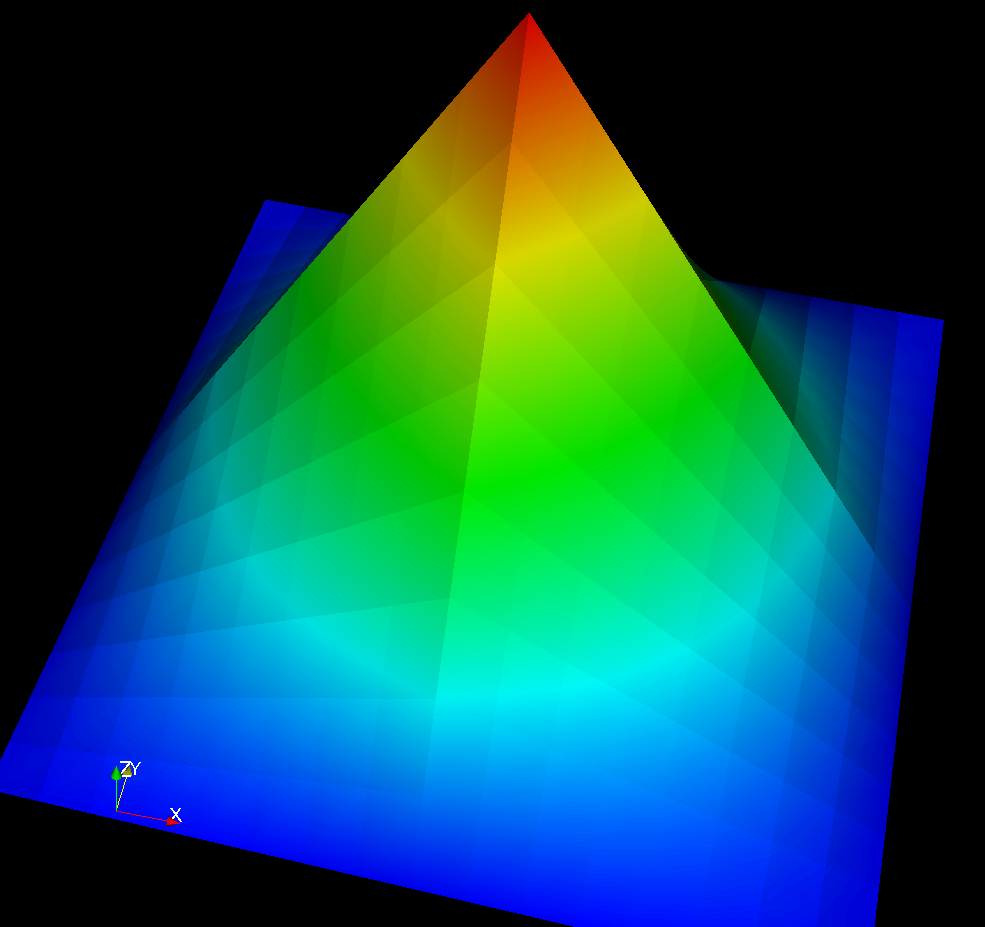
\includegraphics[width=0.65\textwidth]{./EPS/q1}
\end{center}
\end{frame}

Figure \ref{fig:Q1GlobalBasisFunction} shows the result visualized
with ParaView.

\mode<article>{
\begin{figure}
\begin{center}
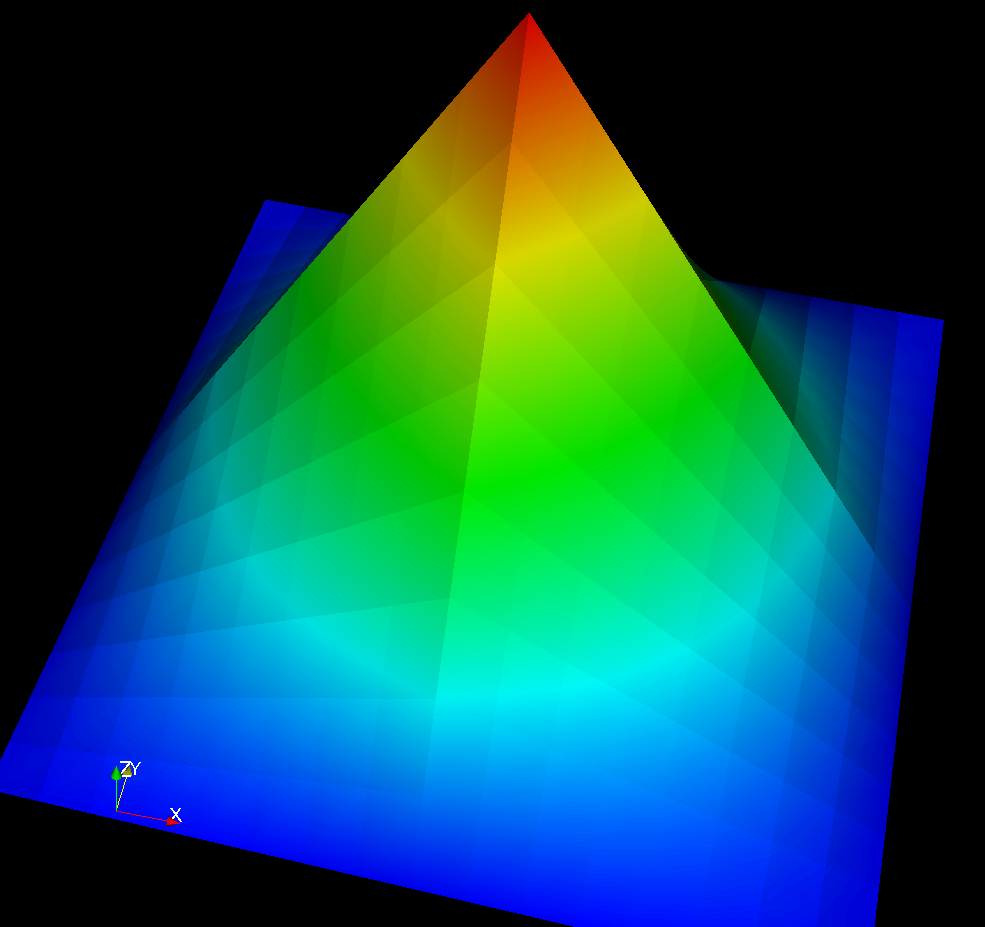
\includegraphics[width=0.5\textwidth]{./EPS/q1}
\end{center}
\caption{$Q_1$ global basis function visualized with ParaView.}
\label{fig:Q1GlobalBasisFunction}
\end{figure}
}

\subsection{Grid Functions}

\mode<article>{
\begin{figure}
\begin{center}
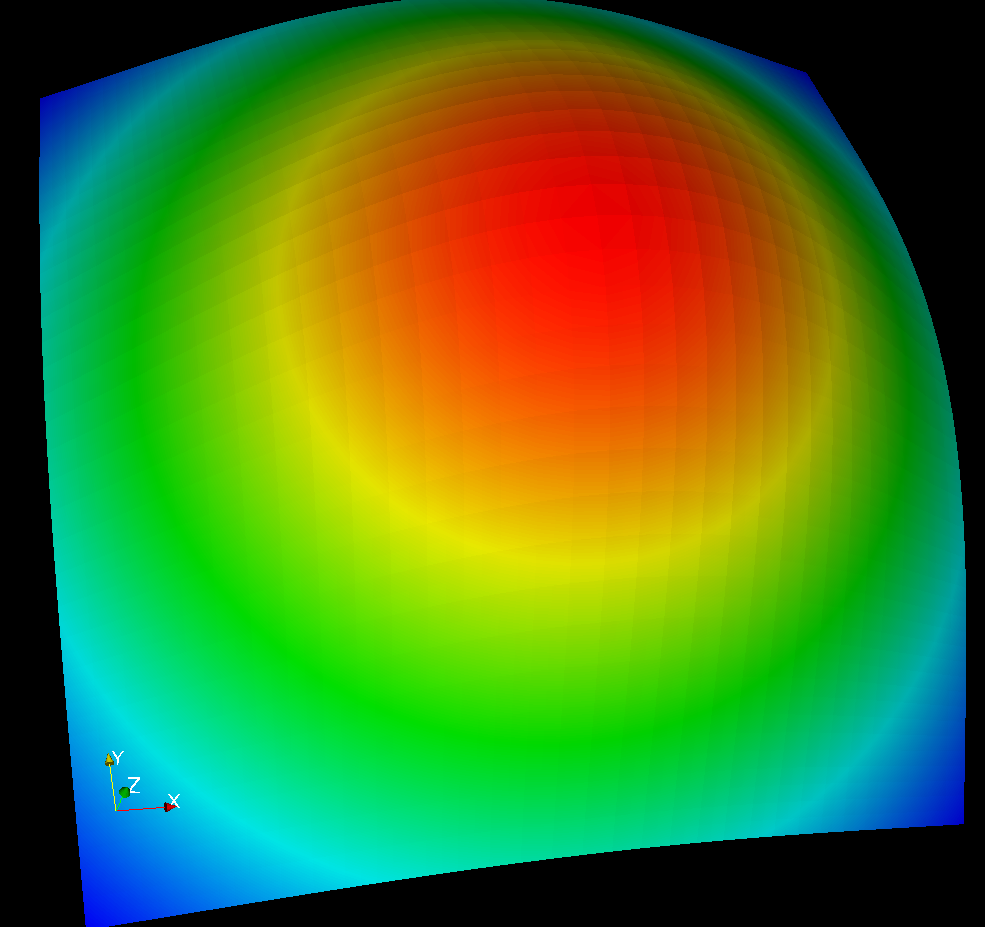
\includegraphics[width=0.5\textwidth]{./EPS/q1interpolate}
\end{center}
\caption{Interpolation of $\exp(-3\|x-c\|^2)$ with $Q_1$ elements.}
\label{fig:Q1Interpolation}
\end{figure}
}

\begin{frame}<article>
\frametitle{Functions}
Often one wants to prescribe functions for initial or boundary
conditions.

PDELab offers several classes to represent functions:
\begin{itemize}
\item \lstinline{Dune::PDELab::FunctionInterface} is the interface for general
functions $$u : \mathbb{D}^n \to \mathbb{K}^m, \qquad x \mapsto y.$$ 
\item \lstinline{Dune::PDELab::GridFunctionInterface} is the interface
for functions defined on a grid:
$$u : E_h^0 \times \mathbb{D}^n \to \mathbb{K}^m, \qquad
(e,\hat{x}) \mapsto y.$$
$\hat{x}$ is on the \textit{reference element}.
\item \lstinline{Dune::PDELab::BoundaryGridFunctionInterface} is the
interface for \textit{grid functions} living on the boundary:
$$u : (E_h^1\text{``$\cap\partial\Omega$''}) \times \mathbb{D}^{n'} \to \mathbb{K}^m, \qquad
(f,\hat{x}) \mapsto y.$$
\item Functions offer the same \lstinline{Traits} as the local basis.
\end{itemize}
\end{frame}


\begin{frame}<article>
\frametitle{Useful Adapters and Base Classes}
There are various useful adapters and base classes:

\lstinline{Dune::PDELab::DiscreteGridFunction}: Takes a scalar
\lstinline{Dune::PDELab::GridFunctionSpace}
and a coefficient vector and makes a scalar grid function out
of it.

\lstinline{Dune::PDELab::VectorDiscreteGridFunction}: Takes a 
\lstinlinegrid{Dune::PDELab::PowerGridFunctionSpace}
and a coefficient vector and makes a vector valued grid function out
of it.

\lstinline{Dune::PDELab::VTKGridFunctionAdapter}: Takes a grid
function and makes a VTK function out of it (this is the input
for \lstinline{VTKWriter}). These two classes have been used already above.

\lstinline{Dune::PDELab::AnalyticGridFunctionBase}: Implements
grid function interface from global function by deriving from it.
This class will be used shortly.

\end{frame}

\begin{frame}<article>
\frametitle{Less Useful Adapters}
\lstinline{Dune::PDELab::FunctionToGridFunctionAdapter}: Takes a global
function and makes a grid function out of it.

\lstinline{Dune::PDELab::GlobalFunctionToLocalFunctionAdapter}:
Takes a global function and an element and provides evaluation
w.r.t.~reference element.

\lstinline{Dune::PDELab::GridFunctionToLocalFunctionAdapter}:
Takes grid function and element, acts as function on the
reference element.

\lstinline{Dune::PDELab::SelectComponentAdapter}. Takas
vector-valued function and component number and provides a scalar function.

\lstinline{D...::BoundaryGridFunctionSelectComponentAdapter}:
Same for boundary grid functions.

\lstinline{Dune::PDELab::PiolaBackwardAdapter}: Takes global
vector-valued function, makes grid function tranformed back to
reference element.

For more details see \lstinline{dune/pdelab/common/function.hh}.
\end{frame}

%\begin{frame}<presentation>[fragile,allowframebreaks,allowdisplaybreaks]
%\frametitle<presentation>{\texttt{AnalyticGridFunctionBase} Example Listing}
%\framesubtitle<presentation>{File \texttt{examples/analyticfunction.hh}}
%\lstinputlisting[basicstyle=\scriptsize,numbers=left, 
%numberstyle=\tiny, numbersep=5pt]{../../examples/analyticfunction.hh}
%\end{frame}
\mode<article>{
\begin{Lst}[File examples/analyticfunction.hh] \mbox
\nopagebreak
\lstinputlisting[basicstyle=\scriptsize,numbers=left, 
numberstyle=\tiny, numbersep=5pt]{../../examples/analyticfunction.hh}
\end{Lst}}

\begin{frame}<article>
\frametitle{Generic Interpolation}
Interpolation of a finite element function from a given function is
now generic.
\end{frame}

%\begin{frame}<presentation>[fragile,allowframebreaks,allowdisplaybreaks]
%\frametitle<presentation>{Generic Interpolation Listing}
%\framesubtitle<presentation>{File \texttt{examples/q1interpolate.hh}}
%\lstinputlisting[basicstyle=\scriptsize,numbers=left, 
%numberstyle=\tiny, numbersep=5pt]{../../examples/q1interpolate.hh}
%\end{frame}
\mode<article>{
\begin{Lst}[File examples/q1interpolate.hh] \mbox
\nopagebreak
\lstinputlisting[basicstyle=\scriptsize,numbers=left, 
numberstyle=\tiny, numbersep=5pt]{../../examples/q1interpolate.hh}
\end{Lst}}

%\begin{frame}<presentation>
%\frametitle<presentation>{Visualization of the Result}
%\begin{center}
%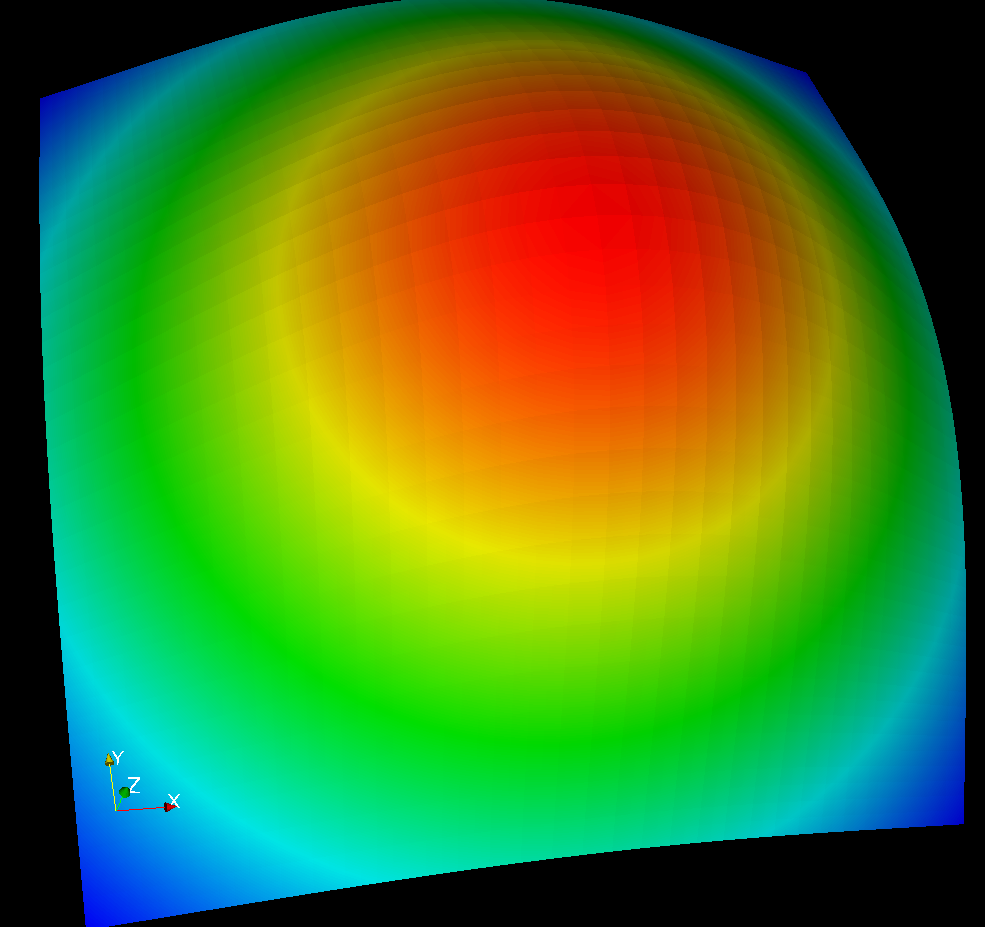
\includegraphics[width=0.65\textwidth]{./EPS/q1interpolate}
%\end{center}
%\end{frame}

\subsection{Interpolation Error Example}

\begin{frame}<article>
\frametitle{Interpolation Error Example}
Now, we do a little example that shows how one can work with global
finite element functions.

For a given function $u$ and its interpolant $u_h\in
U_h(\mathbb{T}_h)$ we want to compute the $L_2$ interpolation error 
\begin{equation*}
\begin{split}
\|&u-u_h\|_{L_2(\Omega)} = \int_\Omega (u-u_h)^2\, dx 
= \sum_{e\in E_h^0} \int_{\Omega_e} (u-u_h)^2\, dx \\
&= \sum_{e\in E_h^0} \int_{\hat{\Omega}_e} \left(u(\mu_e(\hat{x})) -
u_h(\mu_e(\hat{x})) \right)^2 \text{det} \nabla\mu_e(\hat{x}) \,
d\hat{x}\\
&= \sum_{e\in E_h^0} \sum_{j=0}^{q(e)-1} w_{e,j} \left( u(\mu_e(\hat{x}_{e,j})) -
u_h(\mu_e(\hat{x}_{e,j})) \right)^2 \text{det} \nabla\mu_e(\hat{x}_{e,j}) \,
d\hat{x} \text{ $+$ error}\\
&= \sum_{e\in E_h^0} \sum_{j=0}^{q(e)-1} w_{e,j} \left(u(\mu_e(\hat{x}_{e,j})) -
\sum_{i=0}^{k(e)-1}(\mathbf{u})_{g(e,i)} \hat\phi_{e,i}(\hat{x}_{e,j}) \right)^2  
\text{det} \nabla\mu_e(\hat{x}_{e,j}) \,  
d\hat{x} \text{ $+$ error} .
\end{split}
\end{equation*}
\end{frame}

\begin{frame}<article>
\frametitle<presentation>{Interpolation Error Example}
In the following code example the
function \lstinline{l2interpolationerror} is parametrized by
\begin{itemize}
\item \lstinline{U}: Type for a function. 
\item \lstinline{GFS}: Type for a grid function space.
\item \lstinline{X}: Type for a coefficient vector.
\end{itemize}
The local function space
\lstinline{GFS::LocalFunctionSpace} in line \ref{l2int:lfs} is a type 
exported by a grid function space which
\begin{itemize}
\item is bound to an element $e$ later in line \ref{l2int:bind},
\item provides the local finite element for that element $e$ ,
\item provides the local to global map $g(e,\cdot)$ for that element,
\item can read, write and add degrees of freedom of element $e$.
\end{itemize}
\lstinline{Dune::QuadratureRule} in line \ref{l2int:quad} provides
quadrature rules for many element types, dimensions and orders.
\end{frame}

%\begin{frame}<presentation>[fragile,allowframebreaks,allowdisplaybreaks]
%\frametitle<presentation>{Interpolation Error Listing}
%\framesubtitle<presentation>{File \texttt{examples/l2interpolationerror.hh}}
%\lstinputlisting[basicstyle=\scriptsize,numbers=left, 
%numberstyle=\tiny, numbersep=5pt]{../../examples/l2interpolationerror.hh}
%\end{frame}
\mode<article>{
\begin{Lst}[File examples/l2interpolationerror.hh] \mbox
\nopagebreak
\lstinputlisting[basicstyle=\scriptsize,numbers=left, 
numberstyle=\tiny, numbersep=5pt]{../../examples/l2interpolationerror.hh}
\end{Lst}}

Next comes the driver that uses the generic $L_2$ interpolation error
function.

%\begin{frame}<presentation>[fragile,allowframebreaks,allowdisplaybreaks]
%\frametitle<presentation>{Interpolation Error Driver Listing}
%\framesubtitle<presentation>{File \texttt{examples/q1interpolationerror.hh}}
%\lstinputlisting[basicstyle=\scriptsize,numbers=left, 
%numberstyle=\tiny, numbersep=5pt]{../../examples/q1interpolationerror.hh}
%\end{frame}
\mode<article>{
\begin{Lst}[File examples/q1interpolationerror.hh] \mbox
\nopagebreak
\lstinputlisting[basicstyle=\scriptsize,numbers=left, 
numberstyle=\tiny, numbersep=5pt]{../../examples/q1interpolationerror.hh}
\end{Lst}}

\begin{frame}<article>[fragile]
\frametitle{$Q_1$ Interpolation Error Results}
Evaluating the interpolaton error for our $Q_1$ basis for different
levels of refinement produces the following result:
\begin{lstlisting}[basicstyle=\scriptsize]
interpolation error:        1 elements 4.63081768e-01
interpolation error:        4 elements 1.02612039e-01
interpolation error:       16 elements 3.03000305e-02
interpolation error:       64 elements 7.77518775e-03
interpolation error:      256 elements 1.95618596e-03
interpolation error:     1024 elements 4.89819655e-04
interpolation error:     4096 elements 1.22503221e-04
interpolation error:    16384 elements 3.06288243e-05
interpolation error:    65536 elements 7.65739477e-06
interpolation error:   262144 elements 1.91436048e-06
interpolation error:  1048576 elements 4.78590858e-07
\end{lstlisting}
Obviously, we get second order approximation.
\end{frame}

\begin{frame}<article>
\frametitle{Modification for $Q_2$}
Now it is very easy to compute the interpolation error for other
function spaces.

Just replace \lstinline{Q1LocalFiniteElementMap}
with \lstinline{Dune::PDELab::Q22DLocalFiniteElementMap} in
lines \ref{l2int:q2} and \ref{l2int:q22}!
\end{frame}

%\begin{frame}<presentation>[fragile,allowframebreaks,allowdisplaybreaks]
%\frametitle<presentation>{$Q_2$ Interpolation Error Driver Listing}
%\framesubtitle<presentation>{File \texttt{examples/q2interpolationerror.hh}}
%\lstinputlisting[basicstyle=\scriptsize,numbers=left, 
%numberstyle=\tiny, numbersep=5pt]{../../examples/q2interpolationerror.hh}
%\end{frame}
\mode<article>{
\begin{Lst}[File examples/q2interpolationerror.hh] \mbox
\nopagebreak
\lstinputlisting[basicstyle=\scriptsize,numbers=left, 
numberstyle=\tiny, numbersep=5pt]{../../examples/q2interpolationerror.hh}
\end{Lst}}

\begin{frame}<article>[fragile]
\frametitle{$Q_2$ Interpolation Error Result}
And we see third order approximation:
\begin{lstlisting}[basicstyle=\scriptsize]
interpolation error:        1 elements 4.65290291e-02
interpolation error:        4 elements 1.20509875e-02
interpolation error:       16 elements 1.36558258e-03
interpolation error:       64 elements 1.71127393e-04
interpolation error:      256 elements 2.14102072e-05
interpolation error:     1024 elements 2.67692161e-06
interpolation error:     4096 elements 3.34635709e-07
interpolation error:    16384 elements 4.18301070e-08
interpolation error:    65536 elements 5.22878350e-09
interpolation error:   262144 elements 6.53598587e-10
interpolation error:  1048576 elements 8.16998215e-11
\end{lstlisting}
\end{frame}

\cleardoublepage
